\section{Introduction}

As engineers designing sequential decision-making and control algorithms, we have seen enormous, exciting advances in our ability to solve extremely complicated problems without explicit models. I am, of course, talking about the broad machine learning paradigm of Reinforcement Learning (RL). In RL, we are given an environment and an agent, and the goal of the agent is to optimally interact with the environment to learn an optimal policy, which maps the agent's state in the environment to an action to take in the environment \cite{Hussein2017}. In the RL paradigm, there is some goal / task encoded in environmental feedback -- most often, the task that the agent is supposed to complete is given as a reward signal. This means that as the agent takes actions in the environment, the environment rewards the agent, thus implicitly telling the agent what actions to take. This is not the only way to encode the task for the agent; you could alternatively give the agent the policy and ask them to recover the reward function that caused the policy. With this given "expert" policy and the assumption that the environmental actions can be modeled by a generative MDP, the optimal policy and the reward function both specify the same task \cite{NG_IRL}.

Recently, our interest in RL has greatly expanded due to amazing machine learning technology like deep reinforcement learning algorithms. This newfound enthusiasm is tempered by our the lack of explainability of the Deep Neural Networks (DNNs) representing policy / value estimates, their sample inefficiency, their training instability, and the difficult or impossible process of reward design \cite{rlblogpost}.

One of these problems, the great difficulty of designing reward functions to specify the task at hand, is tackled by Learning from Demonstration (LfD) algorithms \cite{Ravichandar2020}. As seen in Fig. \ref{fig: lfd_flow}, the high-level process consists of gathering demonstrations, creating more meaningful representations of those features (i.e. the feature extraction done by all neural networks), learning some representation of the policy from the extracted features, and then refining the policy. In practice, these steps are often combined.

\begin{figure}[htbp]
\centerline{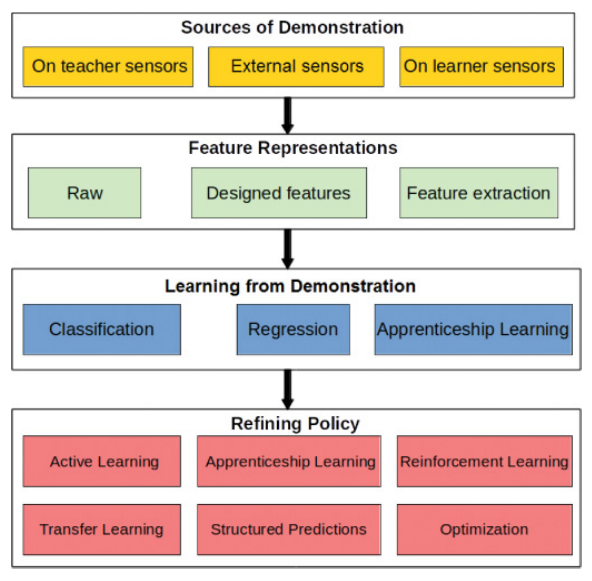
\includegraphics[width=\linewidth]{Figures/lfd_flowchart.png}}
\caption{A flowchart showing the abstract steps and techniques involved in LfD. Reproduced from \cite{Hussein2017}}
\label{fig: lfd_flow}
\end{figure}

\begin{figure}[htbp]
\centerline{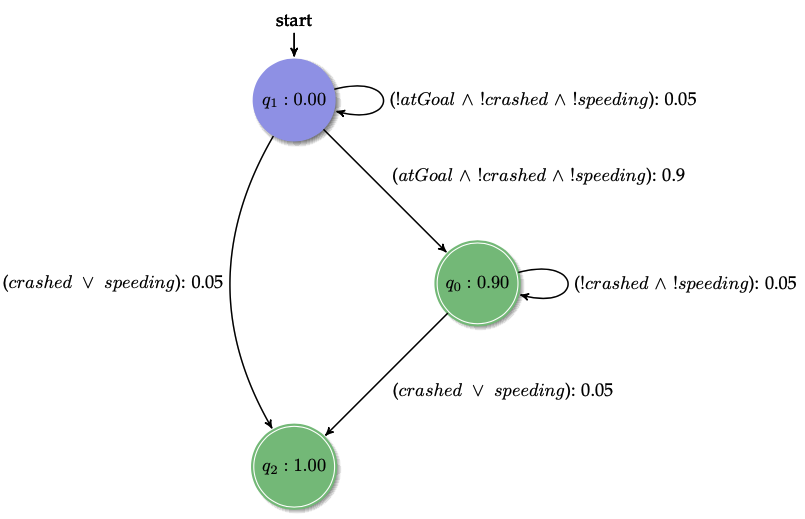
\includegraphics[width=\linewidth]{Figures/PDFA.png}}
\caption{An example of a probabilistic deterministic finite automaton (PDFA) specification for one of my toy autonomous driving scenarios.}
\label{fig: driving_pdfa_spec}
\end{figure}


Another of the stated problems with deep RL, its lack of interpretability, could be solved by going with a model-based approach and combining it with \href{https://en.wikipedia.org/wiki/Formal_methods}{formal methods}. This would fundamentally change the problem from one of defining an agent-environment simulator and specifying the task as a reward function or policy to one of defining a system MDP model and the task specification as a logical structure. This approach, known as formal control synthesis is becoming more and more popular. In his annual review in 2018, Schwarting outlined the progress made in the Verification and Synthesis of decision-making and motion planning algorithms \cite{doi:10.1146/annurev-control-060117-105157}, noting that it was of great interest. He noted that its current limitations are mainly its computational expense and the difficulty in formally specifying desired system behavior. 

Thus, my research is focues on investigating using machine learning to learn high-level, formal (amenable to formal control synthesis) human specifications for system behavior. More specifically, my research consists of first using probabilistic state-machine learning algorithms (e.g. ALERGIA, MDI \cite{prob_state_merging_book}, or RTI(+) \cite{Verwer_PAutomaC}) -- a field of machine learning called Grammatical Inference (GI) -- to learn an automaton model for human demonstrator's specification for the operation of an autonomous system based on observed symbol sequences (traces) representative of desired system behavior. See Fig. \ref{fig: driving_pdfa_spec} for an example of such a specification. These probabilistic state machines are generative and and when sampled from produce traces in the language of the probabilistic automaton. Then, using tools from formal methods, we compose this specification with a model for the autonomous system's dynamics (e.g. \href{https://en.wikipedia.org/wiki/Transition_system}{transition system} or MDP) to obtain a correct-by-construction policy following the learned specification.

Thus, we have now presented a third way to specify the desired behavior of an uncertain decision-making system. We have seen that we can learn to control an uncertain decision-making system with Learning from Demonstration by learning a policy or reward function, or we could model our system explicitly and formally specify its behavior with an automation representation of the task. As of yet, no one has compared these two bleeding edge methodologies for LfD.